\documentclass{book}
\usepackage{amsmath}
\usepackage{amssymb}
\usepackage{amsthm}
\usepackage{bcprules}
\usepackage{tikz}
\usetikzlibrary{fit,shadows,positioning}
\newtheorem{definition}{Definition}
\newtheorem{desiderata}{Desiderata}
\newcommand{\defined}{\downarrow}
\newcommand{\relRx}[1]{\mathrel{R_{#1}}}
\newcommand{\relR}{\relRx{}}
\newcommand{\putr}{\mathit{putr}}
\newcommand{\putl}{\mathit{putl}}
\newcommand{\op}{^\mathit{op}}
\newcommand{\dputr}{\mathord{\Rrightarrow}}
\newcommand{\dputl}{\mathord{\Lleftarrow}}
\newcommand{\discuss}[1]{}
\newcommand{\LIST}{^\star}
\newcommand{\GET}{\ensuremath{\aget}}
\newcommand{\CREATE}{\ensuremath{\acreate}}
\newcommand{\PUT}{\ensuremath{\aput}}
\newcommand{\PUTR}{\ensuremath{\putr}}
\newcommand{\PUTL}{\ensuremath{\putl}}
\newcommand{\missing}{\mathit{missing}}
\newcommand{\aget}{\mathit{get}}
\newcommand{\acreate}{\mathit{create}}
\newcommand{\aput}{\mathit{put}}
\newcommand{\arrow}{\rightarrow}
\newcommand{\ml}[1]{\mathsf{#1}}
\newcommand{\mlinl}{\ml{inl}\ }
\newcommand{\mlinr}{\ml{inr}\ }
\newcommand{\true}{\ml{true}}
\newcommand{\false}{\ml{false}}
\newcommand{\comp}{\mathit{comp}}
\newcommand{\partition}{\mathit{partition}}
\newcommand{\mlfst}{\ml{fst}}
\newcommand{\mlsnd}{\ml{snd}}
\newcommand{\lens}{\leftrightarrow}
\newcommand{\id}{\mathit{id}}
\newcommand{\unit}{{()}}
\newcommand{\Unit}{\mathit{Unit}}
\newcommand{\mlins}[1]{\ml{ins}(#1)}
\newcommand{\mldel}[1]{\ml{del}(#1)}
\newcommand{\mlreorder}[1]{\ml{reorder}(#1)}
\newcommand{\mlmod}[2]{\ml{mod}(#1,#2)}
\newcommand{\partialto}{\rightharpoonup}
\newcommand{\ONE}{\mbox{\bf{1}}}
\newcommand{\init}{\mathit{init}}
\newcommand{\edit}{edit}
\renewcommand{\d}{\textrm{d}}
\newcommand{\dv}{\d v}
\newcommand{\dw}{\d w}
\newcommand{\dx}{\d x}
\newcommand{\di}{\d i}
\newcommand{\dy}{\d y}
\newcommand{\dz}{\d z}
\newcommand{\creater}{\mathit{creater}}
\newcommand{\createl}{\mathit{createl}}
\newcommand{\pdf}[1]{\node[scale=.27]{\pgfimage{pdf/#1}}}
\begin{document}
% TODO

\chapter{Introduction}  % TODO: expand each sentence here to a paragraph
Bidirectional situations are all around us. We synchronize bookmarks, keep
clones of our data on our mobile devices, edit collaboratively, use GUIs to
visualize and modify chunks of our data, etc. So designing tools that
support the creation and maintenance of these transformations is important.

Lots of nice things have been done (e.g. the asymmetric state-based lens
model and its instantiation in Boomerang), but there are many niches where
we might want more targeted support. For decentralized applications, neither
repository is canonical and you want a way to deal with that. For big data,
you want small descriptions of changes. Some data structures aren't most
naturally represented as strings, but as trees, relations, grids, graphs, or
other structures instead.

My thesis will be an exploration of these issues and what can be done to
deal with them; the major unfinished work that I will be proposing is
grid-structured data.

\chapter{Finished work} % TODO: cleanup
\section{Background}
\newif \iftext  \texttrue
\newif \iffull  \fulltrue
\newif \ifdraft \draftfalse
\newif \ifdelta \deltafalse
\newif \iflater \laterfalse  % (for things that we're going to think about later)
\newif \iftikz  \tikztrue
To set the stage, let's review the standard definition of
asymmetric lenses.
%
(Other definitions can be given, featuring weaker or stronger laws, but this
version is widely accepted.)
%
Suppose $X$ is some set of source structures (say, the possible states of a
database) and $Y$ a set of target structures (views of the database).
%
An asymmetric lens from $X$ to $Y$ has two components:
\[
\begin{array}{r@{\ \;}c@{\ \;}l}
\GET &\in& X \arrow Y\\
\PUT &\in& Y \times X \arrow X
\end{array}
\]
The \GET{} component is the forward transformation, a total function from
$X$ to $Y$.  The \PUT{} component takes an old $X$ and a modified $Y$ and
yields a correspondingly modified $X$.  These components
must obey two ``round-tripping'' laws for every $x \in X$ and $y
\in Y$:
%
\infax[GetPut]{
  \PUT\; (\GET \; x)\; x = x
}
\infax[PutGet]{
  \GET\; (\PUT \; y \; x) = y
}
%
It is also useful to be able to create an element of $x$ given just an
element of $y$, with no ``original $x$'' to put it into; in order to handle
this in a
uniform way, each lens is also equipped with a
function $\CREATE\in Y\arrow X$, and we assume one more axiom:
\infax[CreateGet]{
    \GET\; (\CREATE \; y) = y
}

\section{Symmetric lenses}
First, we show that lenses can be generalized from their usual asymmetric
presentation---where one of the structures is always a ``view'' of the
other---to a
fully {\em symmetric} version where each of the two structures may
contain information that is not present in the other.
This generalization is significantly more expressive than any previously
known: although symmetric variants of lenses have been
studied~\cite{Meertens98,stevens2008tat,DBLP:conf/models/Diskin08}, they
all lack a notion of sequential composition of lenses, a significant
technical and practical limitation.
%
As we will see, the extra structure that we need to support composition is
nontrivial; in particular, constructions involving
symmetric lenses need to be proved correct modulo a notion of {\em behavioral
  equivalence}.

Second, we undertake a systematic investigation of the {\em
  algebraic structure} of the space of lenses, using the concepts of
elementary category theory as guiding and organizing principles.  (Our
presentation is self contained, but some prior familiarity
with basic concepts of category theory will be helpful.)

The key  step toward symmetric lenses is the notion
of {\em complements}.  The idea dates back to a famous paper in the
database literature on the view update
problem~\cite{DBLP:journals/tods/BancilhonS81} and was adapted to
lenses in~\cite{Matching10} (and, for a slightly different
definition,~\cite{matsuda2007btb}), and it is quite simple.  If we think of
the
\GET{} component of a lens as a sort of projection function, then we can find
another projection from $X$ into some set $C$ that
keeps all the information discarded by \GET{}.  Equivalently, we can think
of \GET{} as returning two results---an element of $Y$ and an element of
$C$---that together contain all the information needed to reconstitute the
original element of $X$.  Now the \PUT{} function doesn't need a whole $x\in
X$ to recombine with some updated $y\in Y$; it can
just take the complement $c\in C$ generated from $x$ by the \GET, since this
will
contain all the information that is missing from $y$.  Moreover, instead of
a separate
$\CREATE$ function, we can simply pick a distinguished element
$\missing\in C$ and define $\CREATE(y)$ as $\PUT(y,\missing)$.

Formally, an {\em asymmetric lens with complement}
mapping between $X$ and $Y$ consists of a set $C$, a
distinguished element $\missing \in C$, and two functions
\[
\begin{array}{r@{\ \;}c@{\ \;}l}
\GET &\in& X \arrow Y \times C\\
\PUT &\in& Y \times C \arrow X
\end{array}
\]
obeying the following laws for every $x \in X$, $y \in Y$, and $c \in C$:%
\footnote{We can convert back and
forth between the two presentations; in particular, if $(\GET, \PUT,
\CREATE)$ are the components of a traditional lens, then we define a
canonical complement by $C=\{f\in Y{\rightarrow}X\mid \forall
y.\;\GET(f(y))=y\}$. We then define the components $\missing'$, $\GET'$, and
$\PUT'$
of an asymmetric lens with complement as $\missing'=\CREATE$ and
$\GET'(x)=(\GET(x),\lambda y.\PUT(y,x))$ and $\PUT'(y,f)=f(y)$.
\iffull
Going the other way, if $(\aget, \aput, \missing)$ are the components of an
asymmetric lens with complement, we can define a traditional lens by
$\aget'(x) = \mlfst(\aget(x))$ and $\aput'(y,x) = \aput(y,\mlsnd(\aget(x)))$
and $\acreate(y) = \aput(y,\missing)$.
\fi
}
%
\infrule[GetPut]{
  \GET\; x = (y,c)
}{
  \PUT\; (y,c) = x
}
\infrule[PutGet]{
  \GET\; (\PUT \; (y,c)) = (b',c')
}{
  b' = y
}
Note that the type is just ``lens from $X$ to $Y$'': the set
$C$ is an internal component, not part of the externally visible type.
In symbols, $ \mathit{Lens}(X,Y) =
\exists C.\; \{ \mathord{\missing}:\, C,\; \GET:\,X \arrow Y
\times C,\; \PUT:\,Y \times C \arrow X \}$.

Now we can symmetrize.
First, instead of having only \GET{} return a complement, we make \PUT{}
return a complement too, and we take this complement as a second argument
to $\GET$.
%
\iffull
\[
\begin{array}{r@{\ \;}c@{\ \;}l}
\GET &\in& X \times C_Y \arrow Y \times C_X\\
\PUT &\in& Y \times C_X \arrow X \times C_Y
\end{array}
\]
\else
So we have $\GET \in X \times C_Y \arrow Y \times C_X$ and
$\PUT \in Y \times C_X \arrow X \times C_Y$.
\fi
%
Intuitively, $C_X$ is the ``information from $X$ that is discarded by
\GET,'' and $C_Y$ is the ``information from $Y$ that is discarded by
\PUT.''  Next we observe that we can, without loss of generality, use the
same set $C$ as the complement in both directions.  \iffull (This ``tweak''
is actually critical: it is what allows us to define composition of symmetric
lenses.)\fi
\iffull
\[
\begin{array}{r@{\ \;}c@{\ \;}l}
\GET &\in& X \times C \arrow Y \times C\\
\PUT &\in& Y \times C \arrow X \times C
\end{array}
\]
\else
So now we have
$\GET \in X \times C \arrow Y \times C$ and
$\PUT \in Y \times C \arrow X \times C$.
\fi
%
Intuitively, we can think of the combined complement $C$ as $C_X \times
C_Y$---that is, each complement contains some ``private information from
$X$'' and some ``private information from $Y$''; by convention, the \GET{}
function reads the $C_Y$ part and writes the $C_X$ part, while the \PUT{}
reads the $C_X$ part and writes the $C_Y$ part.
%
Lastly, now that everything is symmetric, the \GET{} / \PUT{} distinction is not
helpful, so we rename the functions to \PUTR{} and \PUTL.  This brings us to
our core definition.

\iftikz
\iffull
\begin{figure*}[t!] \centering
\vspace*{-4ex}
\hspace*{-1em}
\begin{tabular}{@{}cc}
  \ifpdf\tikz\pdf{symmetric-minus};\vspace*{-1ex}
  \else \tikz\pdf{symmetric-minus}node[below=8.2ex]{};
  \fi
 &
  \tikz\pdf{symmetric};
  \ifpdf\vspace*{-2ex}\fi
 \\
(a) Initial replicas & (b) Initial complement
\vspace*{4ex} \\
  \ifpdf\tikz\pdf{symmetric-edit};\vspace*{-.7ex}
  \else \tikz\pdf{symmetric-edit}node[below=10ex]{};
  \fi
&
  \tikz\pdf{symmetric-propagatex};
\\
(c) One replica edited & (d) Propagating the edit
\vspace*{3ex}
\\
  \ifpdf\vspace*{3ex}\tikz\pdf{symmetric-edit2};\vspace*{-8ex}
  \else \tikz\pdf{symmetric-edit2}node[below=12.9ex]{};
  \fi
&
  \ifpdf\tikz\pdf{symmetric-propagate2};\vspace*{-1ex}
  \else \tikz\pdf{symmetric-propagate2}node[below=12.9ex]{};
  \fi
\\
(e) Second replica is edited & (f) This change is propagated
\vspace*{1.5ex}
\\
\end{tabular}
\caption{Behavior of a symmetric lens}\vspace*{2ex}
\label{fig:symm}
\end{figure*}
\else
\begin{figure*}[t!] \centering
\vspace*{-4ex}
\hspace*{-1em}
\begin{tabular}{@{}ccc}
  \ifpdf\tikz\pdf{symmetric-minus};\vspace*{-1ex}
  \else \tikz\pdf{symmetric-minus}node[below=8.2ex]{};
  \fi
 &
  \tikz\pdf{symmetric};
  \ifpdf\vspace*{-1ex}\fi
&
  \ifpdf\tikz\pdf{symmetric-edit};\vspace*{-3ex}
  \else \tikz\pdf{symmetric-edit}node[below=10ex]{};
  \fi
 \\
(a) Initial replicas & (b) Initial complement & (c) One replica edited
\vspace*{2ex} \\
  \tikz\pdf{symmetric-propagatex};
&
  \ifpdf\vspace*{3ex}\tikz\pdf{symmetric-edit2};\vspace*{-4ex}
  \else \tikz\pdf{symmetric-edit2}node[below=12.9ex]{};
  \fi
&
  \ifpdf\tikz\pdf{symmetric-propagate2};\vspace*{-1ex}
  \else \tikz\pdf{symmetric-propagate2}node[below=12.9ex]{};
  \fi
\\
(d) Propagating the edit & (e) Second replica is edited & (f) This change is propagated
\vspace*{1ex}
\\
\end{tabular}
\caption{Behavior of a symmetric lens}
\label{fig:symm}
\end{figure*}
\fi
\fi

\begin{definition}[Symmetric lens]
A lens $\ell$ from $X$ to
$Y$ (written $\ell \in X \lens Y$) has three parts:
a set of complements $C$, a distinguished element $\missing \in
C$, and two functions
\begin{eqnarray*}
    \putr &\in& X \times C \to Y \times C\\
    \putl &\in& Y \times C \to X \times C
\end{eqnarray*}
satisfying the following round-tripping laws:
\infrule[PutRL]{\putr(x,c) = (y,c')}{\putl(y,c') = (x,c')}
\infrule[PutLR]{\putl(y,c) = (x,c')}{\putr(x,c') = (y,c')}
When several lenses are under discussion, we use record notation to identify
their parts, writing $\ell.C$ for the complement set of $\ell$, etc.
\end{definition}

\iftext The force of the \rn{PutRL} and \rn{PutLR} laws is to establish some
``consistent'' or ``steady-state'' triples $(x,y,c)$, for which \PUT{}s of $x$
from the left or $y$ from the right will have no effect---that is, will not
change the complement. The conclusion of each rule has the same variable
$c'$ on both sides of the equation to reflect this.  We will use the
equation $\putr(x,c) = (y,c)$ to characterize the steady states.  In
general, a \PUT{} of a new $x'$ from the left entails finding a $y'$ and a
$c'$ that restore consistency.  Additionally, we often wish this
process to involve the
complement $c$ from the previous steady state; as a result, it can be
delicate to choose a good value of $\missing$. This value can often be
chosen compositionally; each of our primitive lenses and lens combinators
specify one good choice for $\missing$.

\iflater\finish{There's a good technical discussion of the options for
  dealing with creation in symmetric.v --- might be worth including it
  here.}\fi \fi

\iffull\else One can imagine other laws.  In particular, the long version of
the paper considers symmetric forms of the asymmetric ``\rn{PutPut}'' laws,
which specify that two \PUT{} operations in a row should have the same
effect as the second one alone.  As with asymmetric lenses, these
laws appear too strong to be desirable in practice.  \fi

%% %
%% We say that lenses $l$ and $l'$ are {\em equivalent} if there exists a
%% relation $\mathord{\equivl} \subseteq C \times \C{l'}$ such that:
%% \infax[MissingC]{l.\missing \equivl l'.\missing}
%% \infrule[PutrC]{
%%   c \equivl c'
%%   \andalso
%%   l.\PUTR (a, c) = (b,c_1)
%%   \andalso
%%   l'.\PUTR (a, c') = (b,c_1')
%% }{
%%   b = b' \ \wedge\   c_1 \equivl c_1'
%% }
%% \infrule[PutlC]{
%%   c \equivl c'
%%   \andalso
%%   l.\PUTL (b, c) = (a,c_1)
%%   \andalso
%%   l'.\PUTL (b, c') = (a,c_1')
%% }{
%%   a = a' \ \wedge\   c_1 \equivl c_1'
%% }

%% With these definitions in place, we can develop some basic
%% structure.  For every set $A$, we can define is an identity lens $\mathit{id}$
%% (with a trivial complement) from $A$ to itself.  If we have a lens $l$
%% from $A$ to $B$ and a lens $l'$ from $B$ to $X$, we can compose them to form
%% a lens $(l;l')$ from $A$ to $X$, using $l.C \times l'.C$ as the complement.
%% %
%% We can also show that, up to equivalence, composition is associative and
%% \emph{id} is its unit---i.e., symmetric lenses form a category.

%% \iffull \else \iftext \finish{Briefly mention the PutPut laws and the fact
%%   that, as usual, they are too strong.} \fi \fi
%% \iffull

\paragraph*{Examples} Figure~\ref{fig:symm} illustrates the use of a
symmetric lens.
%
The structures in this example are lists of textual records describing
composers. The partially synchronized records (a) have a name and two dates
on the left and a name and a country on the right.
%
The complement (b) contains all the information that is discarded by both
$\PUT$s---all the dates from the left-hand structure and all the countries
from the right-hand structure.  (It can be viewed as a pair of lists of
strings, or equivalently as a list of pairs of strings; the way we build
list lenses later actually corresponds to the latter.)  If we add a
new record to the left hand structure (c) and use the $\PUTR$ operation to
propagate it through the lens (d), we copy the shared information (the new
name) directly from left to right, store the private information (the new
dates) in the complement, and use a default string to fill in both the
private information on the right and the corresponding right-hand part of
the complement.  If we now update the right-hand structure to fill in the
missing information and correct a typo in one of the other names
(e), then a $\PUTL$ operation will propagate the edited country to the
complement, propagate the edited name to the other structure, and use the
complement to restore the dates for all three composers.

Viewed more abstractly, the
connection between the information about a single composer in the two tables
is a lens from $X \times Y$ to $Y \times Z$, with complement $X
\times Z$---let's call this lens $e$.  Its \PUTR{} component is given $(x,y)$ as
input and has $(x',z)$ in its complement; it constructs a new complement by
replacing $x'$ by $x$ to form $(x,z)$, and it constructs its output by
pairing the $y$ from its input and the $z$ from its complement to form
$(y,z)$. The \PUTL{} component does the opposite, replacing the $z$ part of
the complement and retrieving the $x$ part.  Then the
top-level lens in Figure~\ref{fig:symm}---let's call it
$e\LIST$---abstractly has type $(X \times Y)\LIST \lens (Y \times Z)\LIST$
and can be thought of as the ``lifting'' of $e$ from elements
to lists.

There are several plausible implementations of
$e\LIST$, with slightly different behaviors when list elements are
added and removed---i.e., when the input and complement arguments to \PUTR{}
or \PUTL{} are lists
of different lengths.  One possibility is to take $e\LIST.C = (e.C)\LIST$
and maintain the invariant that the complement list in the output is the same length as
the input list. When the lists in the input have different lengths, we can
restore the
invariant by either truncating the complement list or padding it with
$e.\missing$.
% \iffull
For example, taking $X = \{a,b,c,\ldots\}$, $Y = \{1,2,3,\ldots\}$, $Z =
\{A,B,C,\ldots\}$, and $e.\missing = (m,M)$, and writing
$\left<a,b,c\right>$ for the sequence with the three elements $a$, $b$, and
$c$, we could have:
\[
\begin{array}{ll}
& \PUTR (\left<(a,1)\right>,\;
         \left<(p,P),(q,Q)\right>)
\\
= &\PUTR (\left<(a,1)\right>,\;
         \left<(p,P)\right>)\mbox{\hspace{7.7em}(truncating)}
\\
= & ( \left<(1,P)\right>,\; \left<(a,P)\right>)
\\ [1.5ex]
& \PUTR (\left<(a,1),(b,2)\right>,\;
         \left<(a,P)\right>)
\\
= &\PUTR (\left<(a,1),(b,2)\right>,\;
         \left<(a,P),(m,M)\right>)\mbox{\qquad(padding)}
\\
= & (\left<(1,P),(2,M)\right>,\;
         \left<(a,P),(b,M)\right>)
\end{array}
\]
% \fi
Notice that, after the first \PUTR{}, the information in the second
element of the complement list $(q,Q)$ is lost.
The second \PUTR{} creates a brand new second element for the list, so the value $Q$ is
gone forever; what's left is the default value $M$.

Another possibility---arguably better behaved---is to keep
  an {\em
  infinite} list of complements.  Whenever we do a \PUT{}, we use (and
update) a prefix of the complement list of the same length as the current
value being \PUT, but we keep the infinite tail so that, later, we have
  values to use when the list being \PUT{} is longer.
%% \finish{Probably we should ``iffull'' the following display once it's been
%%   checked, to save space.}
% \iffull
\[
\begin{array}{ll}
& \PUTR (\left<(a,1)\right>,\;
         \left<(p,P),(q,Q),(m,M),(m,M),\ldots\right>)
\\
= & ( \left<(1,P)\right>,\; \left<(a,P),(q,Q),(m,M),(m,M),\ldots\right>)
\\ [1.5ex]
& \PUTR (\left<(a,1),(b,2)\right>,\;
         \left<(a,P),(q,Q),(m,M),(m,M),\ldots\right>)
\\
= & (\left<(1,P),(2,Q)\right>,\;
         \left<(a,P),(b,Q),(m,M),\ldots\right>)
\end{array}
\]
% \fi

We call the first form the {\em forgetful} list mapping lens and the second
the {\em retentive} list mapping lens.  We will see, later, that the
difference between these two precisely boils down to a difference in the
behavior of the lens-summing operator $\oplus$ in the specification
$e\LIST \simeq \id_\Unit \oplus (e \otimes e\LIST)$ of the list mapping lens.

\iftikz
\begin{figure*}[t!] \centering
\vspace*{-4ex}
\begin{tabular}{@{}ccc}
  \tikz\pdf{sums1};
  &
  \tikz\pdf{sums2};
  \ifpdf\else\vspace*{2ex}\fi
  \\
  (a) Initial replicas & (b) Alphabetizing the right
  \vspace*{2ex} \\
  \tikz\pdf{sums3};
  &
  \tikz\pdf{sums4};
  \ifpdf\else\vspace*{2ex}\fi
  \\
  (c) Inserting Chopin on the left & (d) Deleting Beethoven from the left
\end{tabular}
\caption{Synchronizing lists of sums}
\label{fig:sums}
\end{figure*}
\fi
Figure~\ref{fig:sums} illustrates another use of symmetric lenses. The
structures in this example are lists of categorized data; each name on the
left is either a composer (tagged {\tt inl}) or an author (tagged
{\tt inr}), and each name
on the right is either a composer or an actor.  The
lens under consideration will synchronize just the composers between the two
lists, leaving the authors untouched on the left and the actors untouched on
the right. The synchronized state (a) shows a complement with two lists,
each with holes for the composers.  If we re-order the
right-hand structure (b), the change in order will be
reflected on the left by swapping the two composers. Adding another composer
on the left
(c) involves adding a new hole to each complement; on the left, the location
of the hole is determined by the new list, and on the right it simply shows
up at the end. Similarly, if we remove a composer (d), the
final hole on the other side disappears.

Abstractly, to achieve this behavior we need to define a lens $\comp$
between $(X+Y)\LIST$ and
$(X+Z)\LIST$.  To do this, it is convenient to first define a lens that
connects $(X+Y)\LIST$ and $X\LIST \times Y\LIST$; call this lens $\partition$.
The complement of the $\partition$ is a list of booleans telling whether the
corresponding element of the left list is an $X$ or a $Y$. The $\putr$
function is fairly simple: we separate the $(X+Y)$ list into $X$ and $Y$
lists by checking the tag of each element, and set the complement to exactly
match the tags. For example:
\begin{align*}
\putr(\left<\mlinl a,\mlinl b,\mlinr 1\right>,c) &=
    ((\left<a,b\right>,\left<1\right>),\left<\false,\false,\true\right>) \\
\putr(\left<\mlinl a,\mlinr 1,\mlinl b\right>,c) &=
    ((\left<a,b\right>,\left<1\right>),\left<\false,\true,\false\right>)
\end{align*}
These examples demonstrate that $\putr$ ignores the complement entirely,
fabricating a completely new one from its input. The $\putl$ function, on
the other hand, relies entirely on the complement for its ordering
information. When there are extra entries (not accounted for by the
complement), it adds them at the
end. Consider taking the output of the second $\putr$ above and
adding $c$ to the $X$ list and $2$ to the $Y$ list:
\\[1.5ex]
\noindent\begin{tabular}{l}
$\putl((\left<a,b,c\right>,\left<1,2\right>),\left<\false,\true,\false\right>) =$ \\
\qquad$(\left<\mlinl a,\mlinr 1,\mlinl b,\mlinl c,\mlinr 2\right>,$ \\
\qquad$\left<\false,\true,\false,\false,\true\right>)$
\end{tabular}
\\[1.5ex]
\noindent The $\putl$ fills in as much of the beginning of the list as it
can, using the complement to indicate whether to draw elements from $X\LIST$
or from $Y\LIST$.  (How the remaining $X$ and $Y$ elements are interleaved
is a free choice, not specified by the lens laws, since this case only
arises when we are {\em not} in a round-tripping situation. The strategy
shown here, where all new $X$ entries precede all new $Y$ entries, is just
one possibility.)

Given $\partition$, we can obtain $\comp$ by composing three lenses in
sequence: from $(X+Y)\LIST$ we get to $X\LIST \times Y\LIST$ using
$\partition$, then to $X\LIST \times Z\LIST$ using a variant of the lens $e$
discussed above, and finally to $(X+Z)\LIST$ using a ``backwards''
$\partition$.

\iffull

\section{Edit lenses}

\begin{figure}
    \begin{center}
        \vspace*{-2ex}
        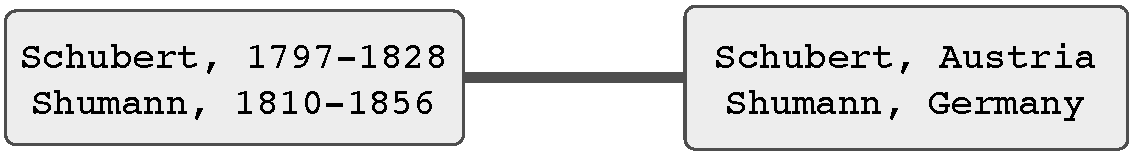
\includegraphics[width=75mm]{images/ex1-init.pdf} \\
        (a) initial replicas \\[1.5ex]
        
\includegraphics[width=75mm]{images/ex1-1.pdf} \\
        (b) a new composer is added to one replica \\[2ex]
        
\includegraphics[width=75mm]{images/ex1-2.pdf} \\
        (c) the lens adds the new composer to the other replica \\[1.5ex]
        
\includegraphics[width=75mm]{images/ex1-3.pdf} \\
        (d) the curator makes some corrections \\[.8ex]
        
\includegraphics[width=75mm]{images/ex1-4.pdf} \\[-3ex]
        (e) the lens transports a small edit \\[1.5ex]
        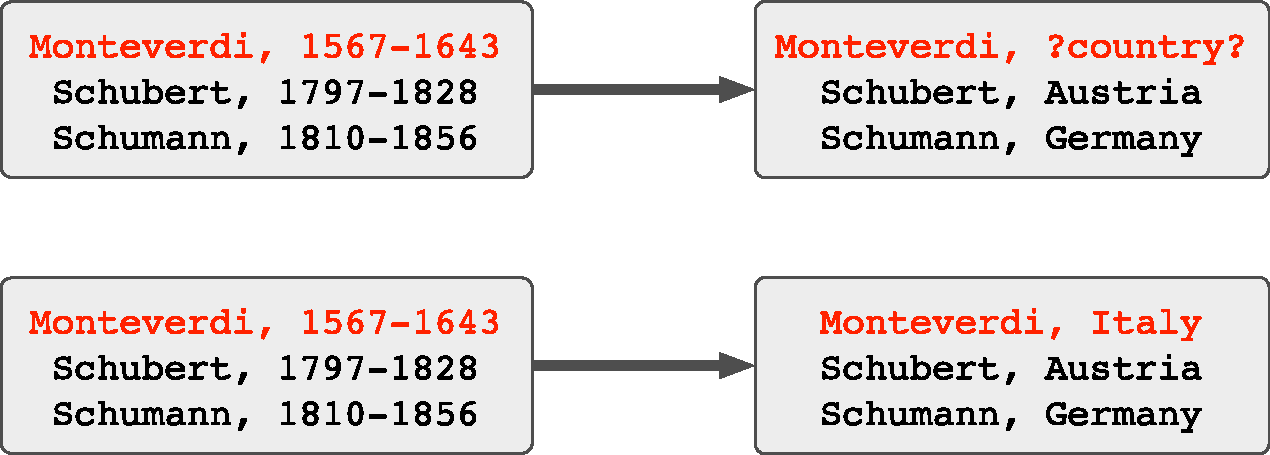
\includegraphics[width=75mm]{images/ex1-5.pdf} \\
        (f) two different edits with the same effect on the left
    \end{center}
\iflater
\discuss{Change the font everywhere to sf}
\fi
    \caption{A simple (complement-less) {\edit} lens in action.}
    \label{fig:example-simple}
\end{figure}

Before diving into technicalities, let's take a brief tour of the main
ideas via some examples.
%
Figure~\ref{fig:example-simple} demonstrates a simple use of {\edit} lenses
to synchronize two replicas.\footnote{We use the word ``synchronize''
  informally to mean simply ``maintain a correspondence between two replicas
  by propagating edits in both directions.''  A full-blown synchronization
  tool would also include, at a minimum, some mechanism for dealing with
  conflicts between disconnected edits to the two structures, which is
  outside the scope of this paper.  \iffull Note, though, that we go beyond most
  synchronization tools in allowing the replicas to be structured
  differently and to share only a part of their information.\fi}  In part (a),
we see the initial replicas, which are in a synchronized state.  On the
left, the replica is a list of records describing composers' birth and death
years; on the right,  a list of records describing the same
composers' countries of origin.  In part (b), the user interacting with the
left-hand replica decides to add a new composer, {\sf Monteverdi}, at the
end of the list.  This change is described by the edit script
{\sf
ins(3); mod(3, (``Monteverdi'', ``1567-1643''))}.
The script says to first
\emph{insert} a dummy record at index three, then \emph{modify} this record by
replacing the left field with ``{\sf Monteverdi}'' and replacing the
right field with ``{\sf 1567-1643}''.  (One could of course imagine other edit
languages where the insertion would be done in one step.  We represent it
this way because this is closer to how our generic ``container mapping''
combinator will do things.)  The
lens connecting the two replicas now converts this edit script into a
corresponding edit
script that adds {\sf Monteverdi} to the right-hand replica, shown in part (c):
{\sf
ins(3); mod(3, (``Monteverdi'', \ONE))}.
Note that the translated {\sf mod} command overwrites the name component but
leaves the country component with its default value, ``{\sf
  ?country?}.''  This is the best it can do, since the edit was in
the left-hand replica, which doesn't mention countries.
%
Later, an eagle-eyed editor notices the missing country information and
fills it in, at the same time correcting a spelling error in {\sf
  Schumann}'s name, as shown in (d). In part (e), we see that the lens
discards the country information when
translating the edit from right to left, but propagates the spelling
correction.

Of course, a particular new replica state can potentially be
achieved by many different edits, and these edits may be translated differently.
%
Consider part (f) of Figure~\ref{fig:example-simple}, where the left-hand
replica ends up with a row for {\sf Monteverdi} at the beginning of the
list, instead of at the end. Two edit scripts that achieve this
effect are shown. The upper script deletes
the old {\sf Monteverdi} record and inserts a brand new one (which happens
to have
the same data) at the top; the lower script rearranges the order of the
list.  The translation of the upper edit leaves {\sf Monteverdi} with a
default country, while the lower edit is translated to a
rearrangement, preserving all the information associated with {\sf
  Monteverdi}.

We do not address the question of where these edits come from or who
decides, in cases like part (f), which of several possible edits is
intended.  As argued in~\cite{Matching10}, answers to these questions will
tend to be intertwined with the specifics of particular editing and/or
diffing tools and will tend to be messy, heuristic, and
domain-specific---unpromising material for a foundational theory.  Rather,
our aim is to construct a theory that shows how edits, however
generated, can be translated between replicas of different shapes.

\iflater\finish{A lot of people got lost at this point.  We need to go much more
  gently.  (In particular, start with a roadmap.)  It would help to rename
  $X,Y,Z$ to something more mnemonic.}\fi

Abstractly, the lens we are discussing maps between structures of the form
$(X \times Y)^*$ and ones of the form $(X \times Z)^*$, where $X$ is the set
of composer names, $Y$ the set of date strings, and $Z$ the set of
countries.  We want to build it compositionally---that is, the whole lens
should have the form $\ell^*$, where $*$ is a ``list mapping'' lens
combinator and $\ell$ is a lens for translating edits to a
single record---i.e., $\ell$ is a lens from $X \times Y$ to $X \times Z$.
Moreover, $\ell$ itself should be built as the product $\ell_1 \times
\ell_2$ of a lens $\ell_1 \in X \to X$ that translates composer edits
verbatim, while $\ell_2$ is a ``disconnect'' lens that maps every edit on
either side to a trivial identity edit on the other side.

In analogous fashion, the edit languages for the top-level structures will
be constructed compositionally.  The set of edits for structures of the form
$(X \times Y)^*$, written $\partial ((X \times Y)^*)$, will be defined
together with the list constructor $*$.  Its elements will have the form
$\mlins{i}$ where $i$ is a position, $\mldel{i}$,
$\mlreorder{i_1,\ldots,i_n}$ where $i_1,\ldots,i_n$ is a permutation on
positions (compactly represented, e.g. as a branching program),
\iflater\discuss{people will be suspicious here---how do we know we
  can represent it compactly?}\fi and $\mlmod{p}{\dv}$, where $\dv \in
\partial (X\times Y)$ is an edit for $X \times Y$ structures.  Pair edits
$\dv \in \partial (X \times Y)$ have the form $\partial X \times
\partial Y$, where $\partial X$ is the set of edits to composers and
$\partial Y$ is the set of edits to dates.  Finally, both $\partial
X$ and $\partial Y$ are sets of primitive ``overwrite edits'' that completely
replace one string with another, together with an identity edit $\ONE$
that does nothing at all; so $\partial X$ can be just $\{\unit\} + X$ (with
$\ONE = \mlinl\unit$) and similarly for $Y$ and $Z$.

%% We write $\ONE$ instead of $\mlinl\ONE$ and {\sf
%%   ``x''} instead of $\mlinr x$ in contexts where it is clear that an edit of
%% this form is expected.

%% We can represent an edit to an element of $X \times Y$ as a pair of
%% edits to $X$ and $Y$; that is, $\partial(X \times Y) = \partial X \times
%% \partial Y$.  The application function $\odot_{X \times Y}$ simply applies
%% each of the component edits to the appropriate parts of the
%% product:
%% \iffull \[ \else $ \fi
%% (\dx,\dy) \odot_{X \times Y} (x, y) = (\dx \odot_X x, \dy \odot_Y y)
%% \iffull .\] \else $. \fi
%% We sometimes write $\mlonl\dx$ as an alias for $(\dx,\ONE)$ when we want to
%% emphasize that a particular edit affects only one part of a tuple, and
%% similarly for $\mlonr\dy$.

Our lens $\ell^*$ will consist of two components---one for transporting edits
from the left side to the right, written $(\ell^*).\dputr \in \partial(X
\times Y)^* \to \partial(X \times Z)^*$,\footnote{The symbol $\dputr$ is
  pronounced ``put an edit through the lens from left to right,'' or just
  ``put right.''  It is the {\edit}-analog of the $\putr$ function of the
  state-based symmetric lenses in~\cite{HofmannPierceWagner10} and the
  $\PUT$ function of the state-based asymmetric lenses
  in~\cite{Focal2005,Boomerang07}.} and another for transporting
edits from right to left, written $(\ell^*).\dputl \in \partial(X \times
Z)^* \to \partial(X \times Y)^*$.
%

%% The next step is to lift this translation to lists.  There are two kinds of
%% edits to lists in the example\finish{why is it this way?}:
%% \emph{rearrangements}, which modify the
%% structure of the list via insertions of dummy elements, deletions,
%% reorderings (but which do not modify the elements themselves), and
%% \emph{modifications} of the values in the list using the underlying element
%% edits (which do not affect the list structure or order).  We already know
%% how to translate modifications, and rearrangements are easy because the list
%% structure is the same on both sides.  Putting these observations together
%% gives us a translation function $\ell^*.\dputr \in \partial((X\times Y)^*)
%% \to \partial((X \times Z)^*)$ for list edits (the $\dputl$ function is
%% similar):
%% \iffull
%%   \begin{align*}
%%     \ell^*.\dputr(\mlins i) &= \mlins i \\
%%     \ell^*.\dputr(\mldel i) &= \mldel i \\
%%     \ell^*.\dputr(\mlreorder{i_0,\ldots,i_n}) &= \mlreorder{i_0,\ldots,i_n} \\
%%     \ell^*.\dputr(\mlmod ie) &= \mlmod i{\ell.\dputr(e)}
%%   \end{align*}
%% \else
%% \[
%% \begin{array}{lcl}
%%     \ell^*.\dputr(\di) &=& \di \\&& \mbox{if $\di$ is an $\mlins$,
%%     $\mldel$, or $\mlreorder$}\\
%%     \ell^*.\dputr(\mlmod ie) &=& \mlmod i{\ell.\dputr(e)}
%% \end{array}
%% \]
%% \fi
%% \iflater
%% \bcp{Not exactly sure what we want to say about this---cutting from the
%%   short version.}
%% The reader may wonder why we break list insertions into
%% two stages---first inserting a dummy element and then modifying this dummy
%% element with desired data. The ease of writing the above function is
%% the answer: since the former stage does not mention elements of the list at
%% all, we need not do any translation, and since the latter stage is
%% simply an edit script, we may dispatch to the underlying lens.
%% \fi
%% %% Additionally,
%% %% the breakdown lets us preserve a nice factorization property that we discuss
%% %% in the next section.\bcp{where? refer to it by number?}

\begin{figure}
    \begin{tabular}{c}
        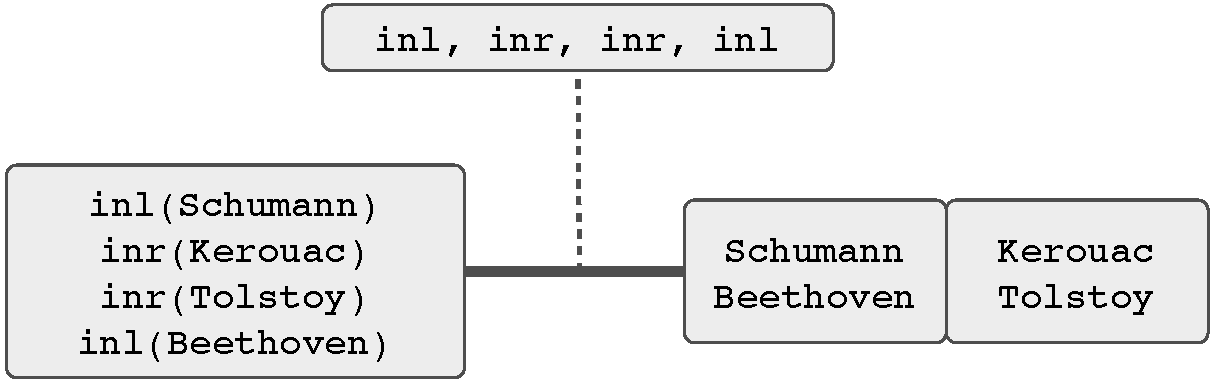
\includegraphics[width=75mm]{images/ex2-0.pdf} \\[.9ex]
        \parbox \linewidth{(a) the initial replicas: a tagged list of composers and authors on
        the left; a pair of lists on the right; a complement storing just
        the tags}
        \\[3ex]
        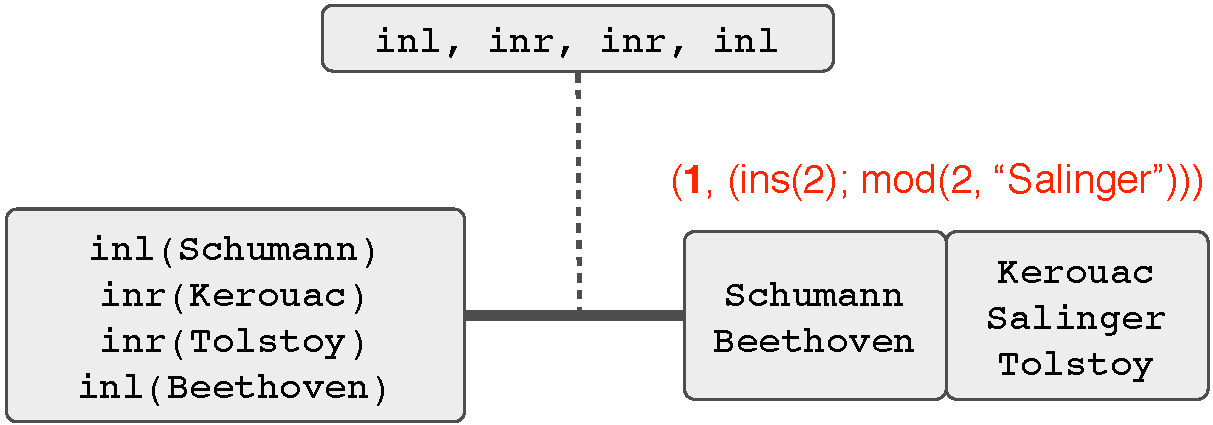
\includegraphics[width=75mm]{images/ex2-1.pdf} \\
        \parbox \linewidth{\begin{center}(b) an element is added to one of
            the partitions\end{center}} \\[2ex]
        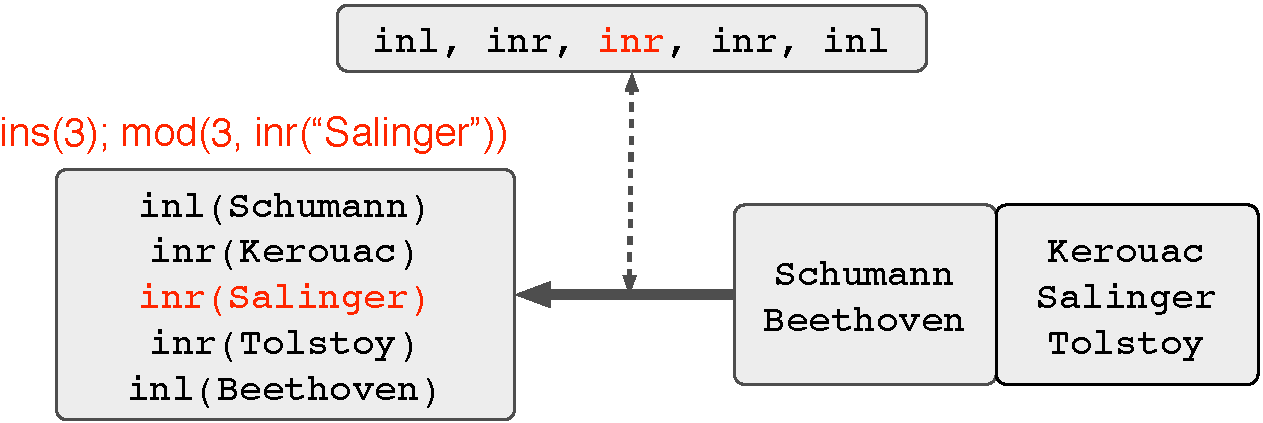
\includegraphics[width=75mm]{images/ex2-2.pdf} \\
        \parbox \linewidth{\begin{center}(c) the complement tells how to translate the
            index\end{center}} \\[.7ex]
    \end{tabular}
    \caption{A lens with complement.}
    \label{fig:example-partition}
\end{figure}

We sometimes need lenses to have a little more structure than this simple
example suggests.
To see why, consider defining a {\em partitioning} lens $p$ between
the sets $\partial((X+Y)^*)$ and $\partial(X^* \times Y^*)$.
Figure~\ref{fig:example-partition} demonstrates the behavior of this lens.
%
In part (a), we show the original replicas: on the left, a single list that
intermingles authors and composers (with {\sf inl/inr} tags showing which is
which), and on the right a pair of homogeneous (untagged) lists, one for
authors and one for composers. Now consider an edit, as in (b), that inserts
a new element somewhere in the author list on the right. It is clear that we
should transport this into an insertion on the left replica, but where, exactly,
should we insert it?  If the $\dputl$ function is given just an
insertion edit for the homogeneous author list and nothing else, there is no
way it can translate this edit into a sensible position in the combined list
on the left, since it doesn't know how the lists of authors and composers
are interleaved on the left.

\iflater\bcp{People were not clear on why the complement was needed.  Also, in this
  example, even with the complement, there is still some arbitrary choice in
  where an inserted element on the right appears in the list on the left.}\fi

The solution is to store a small list, called a {\em complement}, off to the
side, recording the \emph{tags} ($\ml{inl}$ or $\ml{inr}$) from the
original, intermingled list, and pass this list as an extra argument to
translation.  We then enrich the types of the edit translation functions to
accept a complement and return a new complement, so that
%
\iffull \[ \else $ \fi
p.\dputr \in \partial((X+Y)^*) \times C \to \partial(X^* \times Y^*)
\times C
\iffull \] \else $ \fi
and
\iffull \[ \else $ \fi
p.\dputl \in \partial(X^* \times Y^*) \times C \to \partial((X+Y)^*)
\times C
\iffull .\] \else $. \fi
Part (c)
demonstrates the use (and update) of the complement when translating the
insertion.

Note that the complement stores just the {\sf inl/inr} tags, not the actual
names of the authors and composers in the left-hand list.  \iflater\finish{This next
statement made people suspicious---we need to go into more detail.}\fi In general, the
information stored in $C$ will be much smaller than the
information in the replicas; indeed, our earlier example illustrates the
common
case in which $C$ is the trivial single-element set $\Unit$.  The
translation functions manipulate just the complements and the edits, which
are also small compared to the size of the replicas.

%% \finish{Someplace, we need to talk about what happens to edits that don't
%%   make sense on the current state.  There are three possibilities, with a
%%   tradeoff between size of representations and ``accuracy'' of edits:
%%   \begin{itemize}
%%   \item Embed a description of the exact state in the edit and say that the
%%   edit only applies to this state.  This is what Diskin, etc., do.  But it
%%   means that edits are very large.
%%   \item Allow any edit to apply to any state.  Then there are two
%%   sub-possibilities:
%%   \begin{itemize}
%%   \item keep it total but make it behave like the identity (or some other
%%   arbitrary choice) anywhere it doesn't ``make sense''
%%   \item make it partial
%%   \end{itemize}
%%   \end{itemize}
%% }
%% \finish{
%% Old text: Other authors model {\edit}s in other ways; for example, Stevens
%% \finish{citation} chooses functions whose domain and range are equal.
%% Functions are a nice model in some circumstances, but are difficult to
%% inspect: the only operation that can be performed is to apply them to some
%% concrete argument.  Monoids subsume these functions, and some instantiations
%% offer more reflective representations of edits.}

\subsection{Edit Lenses}
\label{sec:semantics}

A key design decision in our formulation of edit lenses is to separate the
{\em description} of edits from the {\em action} of applying an edit to a
state.  This separation is captured by the standard mathematical notions of
{\em monoid} and {\em monoid action}.

\begin{definition}
%% \bcp{why do we say a triple here and in
%%     3.2.3, but other places just name the components (e.g., defn of
%%     category)?}
A \emph{monoid} is a triple $\left<M,\cdot_M,\ONE_M\right>$ of a set
$M$, an associative binary operation $\cdot_M \in M \times M
\to M$, and a unit element $\ONE_M \in M$ --- that is, with $\cdot_M$ and $\ONE_M$ such that
\iffull
\begin{eqnarray*}
x\cdot_M(y\cdot_M z) = (x\cdot_M y) \cdot_M z\\
\ONE_M\cdot_M x = x = x \cdot_M \ONE_M .
\end{eqnarray*}
\else
$x\cdot_M(y\cdot_M z) = (x\cdot_M y) \cdot_M z $ and
$\ONE_M\cdot_M x = x = x \cdot_M \ONE_M$.
\fi
\end{definition}
When no confusion results, we use $M$ to denote both the set and the
monoid, drop subscripts from $\cdot$ and $\ONE$, and write $mn$ for
$m \cdot n$.
%% In more standard terminology, a ``monoid'' in our sense would
%% be called a \emph{partial monoid}\iflater~\cite{partialmonoids}\fi, but
%% since we always work with partial monoids we find it convenient to drop the
%% qualifier.

The unit element represents a ``change nothing'' edit.  Multiplication of
edits corresponds to packaging up multiple edits into a single one
representing their combined effects\iffull{} (this might be useful, for example, for
offline editing)\fi.

Modeling edits as monoid elements gives us great flexibility in
concrete representations.
%
The simplest edit language is a {free monoid} whose elements are just words
over some set of primitive edits and whose multiplication is
concatenation.
%
However, it may be useful to put
more structure on edits, either (a) to allow
more compact representations or (b) to capture the intuition that edits to
different parts of a structure do not interfere with each other and can thus
be applied in any order.
%
The monoid framework can also accommodate more abstract notions of edit.  For
example, the set of all total functions from a set $X$ to itself forms a
monoid, where the multiplication operation is function composition.  This is
essentially the form of edits considered by
Stevens~\cite{stevens2008tat}\iflater\finish{Not just Stevens---we should
  find a few more citations for this idea.}\fi.  \iflater\bcp{Same question for this one.  At a minimum, we should say that we are not dealing with these examples in detail in the rest of the paper.}\fi
%
We mostly focus on the simple case where edit languages are free monoids.
Laws can be added to the product and sum lens constructions, and possibly
for lists and general containers as well.

\begin{definition}
    Given a  monoid $M$ and a set $X$, a \emph{monoid action} on $M$ and $X$
    is a partial function $\odot \in M \times X \partialto X$ satisfying two laws:
\iffull
    \infax{\ONE \odot x = x}
    \infax{(m \cdot n) \odot x = m \odot (n \odot x)}
\else
$\ONE \odot x = x$ and $(m \cdot n) \odot x = m \odot (n \odot x)$.
\fi
\end{definition}
%
As with monoid multiplication, we often elide the monoid action symbol,
writing $mx$ for $m \odot x$.  In standard mathematical terminology, a
monoid action in our sense might instead be called a ``partial monoid
action,'' but since we always work with partial actions we find it
convenient to drop the qualifier.

A bit of discussion of partiality is in order.
Multiplication of edits is a total operation: given two descriptions of
edits, we can always find a description of the composite actions of doing
both in sequence.  On the other hand, {\em applying} an edit to a particular
state may sometimes fail.
%
This means we need to work with expressions and equations involving
partial operations. As usual, any term that contains an undefined
application of an operation to operands is undefined---there is no way of
``catching'' undefinedness. An equation between possibly undefined terms
(e.g., as in the definition above)
means that if either side is defined then so is the other, and their values
are equal (Kleene equality).

Why deal with failure explicitly, rather than keeping edit application total
and simply defining our monoid actions so that applying an edit in a state
where it is not appropriate yields the same state again (or perhaps some
other state)?  One reason is that it seems natural to directly address the
fact that some edits are not applicable in some states, and to have a
canonical outcome in all such cases.  A more technical reason is that, when
we work with monoids with nontrivial equations, making inapplicable edits
behave like the identity is actually
wrong.%
%
\footnote{Here is a slightly contrived example.  Suppose that the set of
  states is natural numbers and that edits have the form $(x\mapsto y)$,
  where the intended interpretation is that, if the current state is $x$,
  then the edit yields state $y$.  It is reasonable to impose the equation
  $(y\mapsto z)\cdot(x\mapsto y) = (x\mapsto z)$, allowing us to represent
  sequences of edits in a compact form.  But now consider what happens when
  we apply the edit $(5\mapsto 7)\cdot(3\mapsto 5)$ to the state $5$.  The
  second monoid action law demands that $((5\mapsto 7)\cdot(3\mapsto 5))
  \odot 5 = (5\mapsto 7)\odot((3\mapsto 5) \odot 5)$, which, by the equation
  we imposed, is the same as $(3\mapsto 7) \odot 5 = (5\mapsto
  7)\odot((3\mapsto 5) \odot 5)$.  But the left-hand side is equal to $5$
  (since the edit $(3\mapsto 7)$ does not apply to the state $5$), while the
  right-hand side is equal to $7$ (since the first edit, $(3\mapsto 5)$, is
  inapplicable to the state $5$, so it behaves like the identity and returns
  $5$ from which $(5\mapsto 7)$ takes us to $7$), so the action law is
  violated.}

However, although the framework allows for the possibility of edits failing,
we still want to know that the edits produced by our lenses will never
actually fail when applied to replica states arising in practice.  This
requirement, corresponding to the {\em totality} property of previous
presentations of lenses~\cite{Focal2005}, is formalized and proven.
In general, we adopt the design principle that partiality
should be kept to a minimum; this simplifies the definitions.

%% Notice that the second law implies that if $m\odot(n\odot x)$ is
%% defined then $m\cdot n$ must be defined and conversely, if $n\odot x$
%% is undefined then $(m\cdot n)\odot x$ must also be undefined for all
%% $m$ even if $m\cdot n$ is defined.

\iflater
\finish{A monoid action is a monoid homomorphism from $M$ to $X \to X$. Can
tie this back to the Stevens work, too, maybe?}
\fi

It is convenient to bundle a particular choice of monoid and monoid
action, plus an initial element, into a single structure:

\begin{definition}
    A \emph{module} is a tuple $\left<X,\, \init_X,\, \partial
    X,\,\odot_X\right>$ comprising a set $X$, an element $\init_X\in X$, a monoid
    $\partial X$, and a monoid action $\odot_X$ of $\partial X$ on $X$.
\end{definition}
If $X$ is a module, we refer to its first component by either
$|X|$ or just $X$, and to its last component by $\odot$ or simple
juxtaposition.

We will use modules to represent the structures connected by lenses.  Before
coming to the definition of lenses, however, we need one last ingredient:
the notion of a {\em stateful homomorphism} between monoids.  As we saw in
the examples, there are situations where the information in an
edit may be insufficient to determine how it should be translated---we may
need to know something more about how the two structures correspond. The
exact nature of the extra information needed varies according to the lens.
%
To give lenses a place to store such auxiliary information, we
follow~\cite{HofmannPierceWagner10} and allow the edit-transforming
components of a lens (the $\dputr$ and $\dputl$ functions) to take a {\em
  complement} as an extra input and return an updated complement as an extra
output.
%
\iflater
\discuss{Not sure there's time to change it now, but I found while writing
  that explanation that the word ``complement'' was quite awkward---I kept
  wanting to say just ``state.''  Moreover, the term is technically a bit
  tenuous now, since what we store is not, in fact, anything like a
  complement in the old database sense.}  \soon{complement becomes correspondence}
\fi

\begin{definition}
Given monoids $M$ and $N$ and a {\em complement set} $C$, a \emph{stateful monoid
  homomorphism} from $M$ to $N$ over $C$ is a function $h \in M \times C \to
N \times C$ satisfying two laws:
%
\vspace*{-1ex}
\infrule{}{h(\ONE_M,c) = (\ONE_N,c)}
\infrule{
         h(m,c) = (n,c') \andalso h(m',c') = (n',c'')
}{
         h(m' \cdot_M m,c) = (n' \cdot_N n,c'')
}
%
These are basically just the standard monoid homomorphism laws, except that
$h$ is given access to some internal state $c \in C$ that it uses (and
updates) when mapping from $M$ to $N$; in the second law, we must thread the
state $c'$ produced by the first $h$ into the second use of $h$, and we
demand that both the result and the effect on the state should be the same
whether we send a composite element $m' \cdot m$ through $h$ all at once or
in two pieces.
\end{definition}

The intended usage of an edit lens is as follows. There are two users,
one holding an element of $X$ the other one an element of $Y$, both
referred to hereafter as {\em replicas}.  Initially, they hold $\init_X$ and
$\init_Y$, respectively, and the lens is initialized with complement
$\ell.\missing$. The users then perform actions and propagate them across
the lens. An action consists of producing an edit $\dx$ (or $\dy$), applying
it to one's current replica $x$ (resp.\ $y$), putting the edit through the lens
to obtain an edit $\dy$ (resp.\ $\dx$), and asking the user on the other
side to apply $\dy$ ($\dx$) to their replica.  In the process, the internal
state $c$ of the lens is updated to reflect the new correspondence between
the two replicas.
\iffull

\fi%
We further assume there is some {\em consistency} relation $K$ between $X$,
$Y$, and $C$, which describes the ``synchronized states'' of the replicas
and complement.  This gives us a natural way to state the totality
requirement discussed above: if we start in a consistent state, make a
successful edit (one that does not fail at the initiating side), and put it
through the lens, the resulting edit is guaranteed (a) to be applicable on
the receiving side and (b) to lead again to a consistent state.  We make no
guarantees about edits that fail at the initiating side: these should not be
put through the lens.

\begin{definition}
A \emph{symmetric edit lens} between modules $X$ and $Y$ consists of a
complement set $C$, a distinguished element $\missing\in C$,
two stateful monoid homomorphisms
\iffull
\[
\begin{array}{lcl}
\dputr &\in& \partial X \times C \to \partial Y \times C \\
\dputl &\in& \partial Y \times C \to \partial X \times C
\end{array}
\]
\else
$\dputr \in \partial X \times C \to \partial Y \times C$ and
$\dputl \in \partial Y \times C \to \partial X \times C$,
\fi
%
%% total functions
%% \[
%% \begin{array}{lcl}
%% \dputr &\in& \partial X \times C \to \partial Y \times C \\
%% \dputl &\in& \partial Y \times C \to \partial X \times C
%% \end{array}
%% \]
%% such that \infax{\dputr(\ONE,c)=(\ONE,c) \qquad \dputl(\ONE,c)=(\ONE,c)}
%% \infrule{ \dputr(\dx_2,c)=(\dy_2,c') \quad
%%   \dputr(\dx_1,c')=(\dy_1,c'') }{ \dputr(\dx_1\ \dx_2,c)=(\dy_1\
%%   \dy_2, c'') } \infrule{ \dputl(\dy_2,c)=(\dx_2,c') \quad
%%   \dputl(\dy_1,c')=(\dx_1,c'') }{ \dputl(\dy_1\ \dy_2,c)=(\dx_1\
%%   \dx_2, c'') }
and a ternary {\em consistency relation}
$K\subseteq |X|\times C\times |Y|$ such that
\begin{itemize}
\item $(\init_X,\missing,\init_Y)\in K$;
\item if $(x,c,y)\in K$ and $\dx\ x$ is defined and $\dputr(\dx,c)=(\dy,c')$, then $\dy\ y$ is also defined and $(\dx\ x,c',\dy\ y)\in K$;
\item if $(x,c,y)\in K$ and $\dy\ y$ is defined and $\dputl(\dy,c)=(\dx,c')$, then $\dx\ x$ is also defined and $(\dx\ x,c',\dy\ y)\in K$.%
%
\iffull
\footnote{One might consider a more general format with ``creation''
  operations $\creater\in X\rightarrow Y\times C$ and symmetrically
  $\createl$.  This format actually arises as a special case of the one
  above by choosing the edit monoids to include operations of the form
  $\text{set}(x)$ for $x\in X$, with action $\text{set}(x)\odot x'=x$. One
  can then define $\creater(x,c) = \dputr(\text{set}(x),c)$.}
\fi
%
\end{itemize}
% \discuss{BCP will add a note about binary consistency relations.  Dual role: Important sanity check on dputs, but also a part of the external specification of the lens.}
\end{definition}

\chapter{Spreadsheets}  Lenses keep two similar pieces of data consistent; as either one evolves,
the lens finds analogous evolutions for the other. However, current lenses
don't generalize smoothly to more than two pieces of data. Spreadsheets
manage many pieces (cells) of data that are related to each other, but they
are generally unidirectional: some cells are special automatically-updated
cells, and the values in these cells are always computed by the system and
cannot be changed by the user. Constraint propagation systems generalize
spreadsheets to be many-directional when possible. However, current systems
do not use old states of the system to guide the computation of new states;
any system state which satisfies the given constraints is allowed.

The goal of the hyperlenses project is to merge the three systems, giving a
way of maintaining constraints between many pieces of data that, when given
an update to some part of the system, finds an ``analogous'' update to the
rest of the system. Below we discuss criteria on which the success of the
hyperlenses project can be judged.

In typical constraint propagation systems, there are variables and
constraints. Constraints may involve any number of variables, and are simply
relations on valuations of those variables. In the following, many of the
relations we care about will be of the form
\[\{(x_1,\ldots,x_m,y_1,\ldots,y_n) \mid f(\overline x) = g(\overline y)\}\]
and so we will simply write these as
$f(\overline x) = g(\overline y)$
when it is clear from context that a relation is expected.

\section{Simple example}
A user might draw up a vacation expenditures spreadsheet that looks like
this:

\begin{tabular}[h]{lrrrr}
    Day     & Travel    & Lodging   & Food  & Total \\
    1       & 750       & 120       & 45    & 915   \\
    2       & 30        & 120       & 18    & 168   \\
    3       & 0         & 120       & 150   & 270   \\
    4       & 15        & 120       & 30    & 165   \\
    5       & 750       & 0         & 15    & 765   \\
    Total   & 1545      & 480       & 258   & 2283  \\
\end{tabular}

Along with the table, we would expect to see some constraints like
\begin{align*}
    \mathrm{Travel}_\mathrm{Total} &=
    \mathrm{Travel}_1+\mathrm{Travel}_2+\mathrm{Travel}_3+\mathrm{Travel}_4+\mathrm{Travel}_5
    \\
    \mathrm{Total}_1 &= \mathrm{Travel_1}+\mathrm{Lodging}_1+\mathrm{Food}_1
\end{align*}
and so on, with ten constraints in all (one each for days 1, 2, 3, 4, 5, and
Total, and one each for categories Travel, Lodging, Food, and Total). Here
are some things a user might want to do with this setup:
\begin{itemize}
    \item The user might go on another vacation, and want to make an
        estimate of how much he spent on food given his credit card balance
        at the end of the trip. To do this, he might update
        $\mathrm{Total}_\mathrm{Total}$ to his balance and look in the
        $\mathrm{Food}_\mathrm{Total}$ cell to get a guess.
    \item The user might like to plan a vacation to a certain
        location with a certain budget; then he could fix the
        $\mathrm{Total}_\mathrm{Total}$ cell and update the travel prices
        for the first and last day's plane tickets to get an estimate of how
        much he can spend on the various other days and categories while
        staying in his budget.
    \item Perhaps the user discovers that he is missing a category for
        entertainment and wants to add a new column, initially populated
        with zeros. He did not keep careful track of his daily spending for
        this on the last vacation, but he knows that in total he spent about
        \$800 on entertainment, so he updates the new
        $\mathrm{Entertainment}_\mathrm{Total}$ cell to 800.
\end{itemize}

\section{Goal statement}
{\bf A hyperlens should be a generalization of both lenses and spreadsheets that
supports high-level planning.}

Hyperlenses should generalize lenses. It should be true that there is a
behavior-preserving embedding of asymmetric, state-based lenses: that is, we
can identify two variables in the hyperlens system whose values correspond
to states of the asymmetric lens' two repositories, and the values in the
hyperlens system evolve in the same way they would evolve when running the
lens itself. Moreover, we demand that there be a ``hyperlens composition''
that preserves this property: the embedding of a composition of lenses is
the composition of their embeddings.

A stretch goal is to generalize symmetric, state-based lenses in a similar
way, and again to find a composition operator (potentially different from
the previous one) that corresponds to symmetric lens composition.

Hyperlenses should generalize spreadsheets. It is unreasonable to demand
that the hyperlens framework be capable of bidirectionalizing all
spreadsheets in a reasonable way. However, on the class of spreadsheets that
can be bidirectionalized, it should be the case that using the corresponding
hyperlens as if it were a unidirectional spreadsheet produces the same
answers as the original spreadsheet would.

A stretch goal is to generalize spreadsheets in the sense that any
spreadsheet can be expressed as a (possibly still unidirectional) hyperlens
with the same behavior.

Hyperlenses should support high-level planning. As with all bidirectional
systems, there will be some updates which can be spread through the
remainder of the system in many ways. Support for high-level planning means
that there is some holistic language (that is, which does not require
intimate knowledge of the structure of the term used to define the
hyperlens) for expressing the relative desirability of the various coherent
updates to the system. The system should then be able to compute the most
desirable update. For example, one such language might be, ``spread as much
of the change as possible to such-and-such a variable''.

% TODO: cite a few use cases with the high-level planning we want for each
\section{Simplistic solutions}
Some particularly simple regimes have already been explored. Four such
regimes are discussed below, but it will be helpful to have a few
conventions in place first.

Fix a linearly ordered set $N$ of names and a universe $U$ of values. Since
we are dealing with partial functions, we will use the convention that
$a = b$ whenever both $a$ and $b$ are undefined or whenever $a$ and $b$ are
defined and identical. Likewise, $a \in b$ means that both $a$ and $b$ are
undefined or they are both defined and $a$ is a member of $b$.

\begin{definition}
    A \emph{valuation} is a finite map from $N$ to $U$.
\end{definition}

We generalize valuation application from names to finite sets of names using
the linear ordering on $N$: whenever $x_1 < \cdots < x_m$ is an increasing
chain, $f(\{x_1,\ldots,x_m\}) = (f(x_1),\ldots,f(x_m))$.

\begin{definition}
    A \emph{constraint} is a finite set $n \subset N$ together with a relation $R
    \subset U^{|n|}$.
\end{definition}

\begin{definition}
    A valuation $f$ \emph{satisfies} constraint $(n,R)$ when $f(n) \in R$.
\end{definition}

\begin{definition}
    The \emph{constraint system graph} induced by a set of constraints is
    the undirected bipartite graph whose nodes are drawn from $N$ in one
    part and constraints in the other, and which has an edge $(v,(n,R))$ iff
    $v \in n$.
\end{definition}

\subsection{Spreadsheets}
% TODO: write about unidirectional methods

\subsection{Tree topology}
% TODO

Lenses correspond to a very strong restriction on graph topology: there are
always exactly two variable nodes with exactly one constraint connecting
them. This makes choosing an update plan particularly simple, since we must
always update the nodes attached to the single constraint.

In fact, this observation generalizes slightly: if the constraint system
graph is a tree and we allow the update of only a single node, then we may
direct the constraint graph by treating the updated node as a root and
update nodes attached to constraints in topological order (provided we
promise not to update a given node's value twice).

\subsection{Linear constraints}
Here is a simple spreadsheet which nevertheless fails the tree-structured
property described previously:
\begin{align*}
    tax &= 0.08*base \\
    total &= base + tax
\end{align*}
Despite the mildly interesting structure of the constraint system graph, it
is still definitely possible to bidirectionalize this spreadsheet.

Suppose each constraint in the spreadsheet is \emph{linear}, that is, has
the form
\[x = b+\sum_ic_iy_i\]
for some constants $b$ and $\bf c$. We can form a \emph{directed} constraint
system graph where the edges for the constraint associated with this
equation point from the $y_i$ and towards the $x$. Then, in addition to the
linearity assumption, we will assume that there are no directed cycles in
the directed constraint system graph and that each node has in-degree at
most one. (Undirected cycles, however, are allowed; for example, the
two-equation spreadsheet above has undirected but not directed cycles in its
directed constraint system graph.) Call nodes with in-degree zero (that is,
nodes with no defining equation) \emph{root nodes}.

Under these assumptions, a simple argument shows that, given a cell in the
spreadsheet, we can write an affine formula which maps the values of root
cells to the value of the given cell. The argument goes by induction on the
length of the longest path from a root cell to the given one, and proceeds
by substituting in affine formulas for each non-root variable at each step.
In fact, we can go a step farther: we can write affine transformations from
root cells to any set of cells. If we manage to give a characterization of
when these affine transformations can be bidirectionalized, then we will
have given an account of how to handle the multi-update problem and relax
the simple structure requirement in the parts of the spreadsheet where only
affine formulae are used.

Thus, we can now frame our problem in another way: what is the right way to
bidirectionalize an affine transformation? Accordingly, we will now step
away from spreadsheets and frame our discussion in linear algebra terms.

A function $\aget \in \R^m \to \R^n$ is affine exactly when there is a matrix
$M$ of dimension $n \times m$ and vector $\mathbf b \in \R^n$ such that $\aget(\x) =
M\x +\mathbf b$.  Affine functions are surjective (and hence bidirectionalizable)
just when $M$ has rank $n$, so we assume this. When $m=n$, $f$ is a
bijection. The put function in this case is particularly boring, because it
ignores the original source:
\[\aput(\x,\y) = M^{-1}(\y-\mathbf b)\]
The more interesting case is when $m>n$, and where each $\y$ is therefore
the image of a nontrivial subspace of $\R^m$. There are many heuristics one
may choose to identify a particular point in this subspace; we choose the
specification:
\[\aput(\x,\y) = \argmin{\x',\aget(\x')=\y}||\x' - \x||\]

\begin{lemma}
    There exists an $m \times n$ matrix $N$ such that
    \[\aput(\x,\y) = \x + N(\y - \aget(\x))\]
    satisfies the specification above.
\end{lemma}
\emph{Proof sketch.} The intuition is that we wish to move as little as
possible in source-space to match the move in target-space. This can be
achieved by minimizing how far we move in the null space of $M$, since
(exactly) these motions result in no motion in target-space.

Take a basis $\{\x_1,\ldots,\x_{m-n}\}$ for the null space of $M$. Then
we will take:
\begin{align*}
    B &= \left[\begin{array}{c}
            \x_1\transpose \\
            \vdots \\
            \x_{m-n}\transpose
        \end{array}\right] \\
    N &= \left[\begin{array}{c}
            M \\
            B
        \end{array}\right]^{-1}
        \left[\begin{array}{c}
            I_n \\
            \mathbf 0_{m-n,n}
        \end{array}\right] \\
\end{align*}
Turning the sketch into a proof involves arguing three things: that the
square matrix in the definition of $N$ is invertible; that $N$ produces a
put function that roundtrips; and that the put function produced by $N$
produces minimal changes. The definition above was crafted so that (assuming
for the moment that $N$ exists) we have $MN = I$, which is used to show the
roundtrip property, and $BN = \mathbf 0$, which is used to show minimality.

% TODO: finish this proof and replace the above sketch, maybe
%\begin{proof}
%    The intuition is that we wish to move as little as possible in
%    source-space to match the move in target-space. This can be achieved by
%    minimizing how far we move in the null space of $M$, since (exactly)
%    these motions result in no motion in target-space.
%
%    Take a basis $\{\x_1,\ldots,\x_{m-n}\}$ for the null space of $M$. Then
%    we will take:
%    \begin{align*}
%        B &= \left[\begin{array}{c}
%                \x_1\transpose \\
%                \vdots \\
%                \x_{m-n}\transpose
%            \end{array}\right] \\
%        N &= \left[\begin{array}{c}
%                M \\
%                B
%            \end{array}\right]^{-1}
%            \left[\begin{array}{c}
%                I_n \\
%                \mathbf 0_{m-n,n}
%            \end{array}\right] \\
%    \end{align*}
%    We must now argue three things: that the square matrix in the definition
%    of $N$ is invertible; that $N$ produces a put function that roundtrips;
%    and that the put function produced by $N$ produces minimal changes. The
%    definition above was crafted so that (assuming for the moment that $N$
%    exists) we have $MN = I$, which is used to show the roundtrip property,
%    and $BN = \mathbf 0$, which is used to show minimality.
%
%    invertible: (TODO)
%
%    roundtrip:
%        \begin{align*}
%            \aget(\aput(\x,\y))
%                &= M(\x+N(\y-M\x-\mathbf b))+\mathbf b & \mbox{definition of }\aget,\aput \\
%                &= MN\y + M\x + \mathbf b - MN(M\x + \mathbf b) & \mbox{rearranging terms} \\
%                &= \y & MN=I
%        \end{align*}
%
%    minimal: (TODO)
%\end{proof}

\subsection{Non-associative composition}
% TODO: pick a better subsection name
% TODO: write

\section{Design axes}

A full solution could reasonably build on either the restrictive constraints
or the restrictive topology solutions given above. Because it seems
difficult to extend the restrictive constraints solution sufficiently to
achieve our top-level goal of embedding all asymmetric, state-based lenses,
the approach of extending the restrictive topology solution seems more
promising. Below, we discuss some of the difficulties that should be addressed
by a successful extension.

There is a distinction between the dynamic and static semantics of a
constraint system graph. Unless specified otherwise, all discussion is of
the static semantics.
\begin{definition} Semantics:
    \begin{description}
        \item[Dynamically ambiguous] means the current set of constraints and
            requested updates have multiple satisfying valuations.
        \item[Dynamically unsolvable] means the current set of constraints and
            requested updates have no satisfying valuations.
        \item[Statically ambiguous] means there is a set of requested updates
            and a set of constraints whose graph is the current one which is
            dynamically ambiguous.
        \item[Statically unsolvable] means there is a set of requested updates
            and a set of constraints whose graph the current one which is
            dynamically unsolvable.
    \end{description}
\end{definition}

\subsection{Sources of ambiguity}
\subsubsection{Intra-constraint ambiguity}
Consider the very simple constraint system which has only one constraint, $z
= x+y$. Giving a value for $z$ gives us a classical ``underconstrained
system'': there are infinitely many choices for $x$ and $y$ that satisfy
this constraint. For example, we might choose to keep $y$ and only update
$x$, we might choose to increase $x$ and $y$ by the same summand, we might
ignore the old values of $x$ and $y$ altogether and make them both be
particular fractions of $z$, we might attempt to preserve the product $x*y$,
etc. In our simple example, when we update the grand total, one reasonable
choice would be to scale all the summands by the same factor the grand total
was scaled by.

More abstractly, we might wish to have some runtime control over how
constraint solutions are being chosen in case there is ambiguity.

\begin{desiderata}
    Have programmer-level control over the resolution of individual
    constraints.
\end{desiderata}
\begin{desiderata}
    Have high-level control over the resolution of individual constraints.
\end{desiderata}

\subsubsection{Cycles and inter-constraint ambiguity}
Above, we discussed the possibility of constraint system graphs with cycles
in them. We observed that in such situations, it may be that no ordering of
the constraints' methods may result in a consistent state; however, there
are also situations where many orderings each result in a consistent state
-- and indeed, the chosen consistent states may even differ. As a very
simple example, consider this system that has some seemingly redundant
variables:
\begin{align*}
    z_1 &= x+y \\
    z_2 &= x+y
\end{align*}
We will assume that each constraint either allows us to update $z_i$ alone
given $x$ and $y$ or allows us to update $z_i$ and $y$ together. The first
constraint uses the update policy
\[(z_1',y') = \left(z_1 + \frac{x'-x}2, y - \frac{x'-x}2\right)\]
which spreads half the change to each variable, while the second constraint
uses the update policy
\[(z_2',y') = \left(z_2 + \frac{x'-x}3, y - \frac{2(x'-x)}3\right)\]
which spreads only a third of the change to $z_1$ and the rest to $y$.
% TODO: picture

Suppose we start from the all-zero valuation and then update $x$ to $6$.
There are (at least) two reasonable update plans that guarantee consistency:
update $z_1$ and $y$ together to $3$ and $-3$, respectively, then update
$z_2$ to $3$, or the symmetric plan that updates $z_2$ and $y$ together to
$2$ and $-4$, then updates $z_1$ to $2$.

\begin{desiderata}
    Provide high-level control over ambiguous cycles.
\end{desiderata}

\subsection{Sources of insolubility}
\subsubsection{Cycles}
Suppose we have three variables, $x$, and $y$, and $z$, and three
constraints, one on each pair of variables. We will allow ourselves to
assume we also have a collection of methods for each individual constraint
that can take an update to one of the variables and produce a value of the
other variable that satisfies the constraint. The question now becomes: can
we take an update to one variable, say, $x$, and produce updates to the
other two that reinstate all three constraints?

The naive approach, where we compute $y$ from our assumed method that
reinstates the $\{x,y\}$ constraint and $z$ from our assumed method that
reinstates the $\{x,z\}$ constraint doesn't necessarily work, since there is
no guarantee that the $y$ and $z$ computed this way satisfy the $\{y,z\}$
constraint.

Consider our simple example above: there are two ``paths'' in the constraint
graph from the $\mathrm{Total}_\mathrm{Total}$ node to the
$\mathrm{Travel}_1$ node, namely via $\mathrm{Total}_1$ and via
$\mathrm{Travel}_\mathrm{Total}$. What we would be asking for is a guarantee
that, for example, the way we choose to spread an update over the category
totals and thereafter over the individual cells is compatible with the way
we choose to spread an update over the day totals and thereafter over the
individual cells. In the case of our simple example, we could certainly
achieve this using arithmetic facts, but in more complicated examples the
way forward is less clear.

\begin{desiderata}
    Handle dynamically solvable cycles.
\end{desiderata}

\subsubsection{Multiple update}
Many constraint propagation systems support the update of multiple variables
simultaneously. As discussed in our simple running example, making a
vacation plan on a budget might involve setting the grand total and the
travel costs all at once. This is distinct from setting them one at a time,
since we want the system to guarantee that all three values can coexist,
whereas when we set them one at a time each update may disrupt the values of
the other two.

\begin{desiderata}
    Identify solvable multiple updates.
\end{desiderata}

\subsection{Other difficulties}

% TODO: motivate why each of these is nice and why each is hard
\begin{desiderata}
    Provide an associative, commutative composition operation.
\end{desiderata}
\begin{desiderata}
    Reinstate coherence in a single pass: for each constraint, execute one
    method at most once.
\end{desiderata}
\begin{desiderata}
    Provide a syntax for basic spreadsheet programming.
\end{desiderata}

\subsubsection{Inter-constraint coordination}
It would be nice if the hyperlens associated with
\begin{align*}
    x &= a+b \\
    y &= x+c
\end{align*}
behaved ``similarly'' to the hyperlens associated with
\begin{align*}
    x &= b+c \\
    y &= a+x
\end{align*}
in the sense that an update to $y$ in either system resulted in the same
updates to $a$, $b$, and $c$. This is nice from a language design point of
view because it means you need not introduce separate $+$ functions for each
arity, and is nice from a usability point of view because it means that
there is no price to pay for modularity: you can split up your code into
whatever units make sense to you and get the same program out.

\begin{desiderata}
    Allow constraints to interact during system update.
\end{desiderata}

\chapter{Related work}  % TODO: why is the citation style (and reference style!) so awful?
\section{Symmetric lenses}
% TODO: cleanup (remove ifs, rework wording so it fits in this document)
\newif \iftext  \texttrue
\newif \iffull  \fulltrue
\newif \ifdraft \draftfalse
\newif \ifdelta \deltafalse
\newif \iflater \laterfalse  % (for things that we're going to think about later)

% If you want to build without tikz, put 
%    \tikzfalse 
% in a separate texdirectives.tex file...
\newif \iftikz  \tikztrue
There is a large literature on lenses and related approaches to
propagating updates between connected structures.  We discuss only the most
closely related work here; good general surveys of the area can be found
in~\cite{FosterThesis,DBLP:conf/icmt/CzarneckiFHLST09}.  Connections to the
literature on {\em view update} in databases are surveyed
in~\cite{Focal2005-shortcite}. \iffull A short version of this paper is available
in~\cite{HofmannPierceWagner10}.\fi

The first symmetric approach to update propagation was proposed by
Meertens~\cite{Meertens98} and followed up \iffull in the context of
model-driven design \fi by Stevens~\cite{Stevens07},
Diskin~\cite{DBLP:conf/models/Diskin08}, and Xiong, et
al~\cite{xiong2009supporting}.
%
Meertens suggests modeling synchronization between two sets
$X$ and $Y$ by a {\em consistency relation} $R\subseteq
X\times Y$ and two {\em consistency maintainers}
$\triangleleft: X\times Y\rightarrow X$ and $\triangleright: X\times Y
\rightarrow Y$ such that $(x\triangleleft y) \relR y$ and
$x \relR (x\triangleright y)$ always hold, and such that $x \relR y$ implies
$x \triangleleft y = x$ and $x \triangleright y = y$.

The main advantage of symmetric lenses over consistency maintainers is
their closure under composition. Indeed, all of the aforementioned
authors note that, in general, consistency maintainers do not compose
and view this as a drawback.
%
Suppose that we have relations $R\subseteq X\times Y$ and
$R'\subseteq Y\times Z$ maintained by $\triangleright,\triangleleft$
and $\triangleright', \triangleleft'$, resp. If we want to construct a
maintainer for the composition $R;R'$, we face the problem that, given
$x\in X$ and $z\in Z$, there is no canonical way of coming up with a
$y\in Y$ that will allow us to use either of the existing maintainer
functions. Concretely, Meertens gives the following counterexample.
Let $X$ be the set of nonempty context free grammars over some alphabet, and let
$Y$ be the set of words over that same alphabet. Let $R\subseteq
X\times Y$ be given by $G \relR x\iff x\in L(G)$. It is easy to define
computable maintainer functions making this relation a constraint
maintainer. Composing this relation with its opposite yields an 
undecidable relation (namely, whether the intersection of two context-free
grammars is nonempty), so there cannot be computable maintainer functions.

We can transform any constraint maintainer into a  symmetric lens as
follows: take the relation $R$ itself (viewed as a set of pairs) as
the complement, and define $\putl(x',(x,y))=(x'\triangleright
y,(x',x'\triangleright y))$ and similarly 
for $\putr$. If we compose such a symmetric lens with its opposite
we obtain $R\times R\op$ as the complement and, for example,
$\putr(x',((x_1,y_1),(y_2,x_2))) = 
(x_2\triangleleft(x'\triangleright y_1), ((x',x'\triangleright
y_1),(x'\triangleright y_1,x_2\triangleleft(x'\triangleright y_1))))$. 
%
For Meertens' counterexample, we would have complements of the form
$((G_1,w_1),(w_2,G_2))$, with $w_1\in L(G_1)$
and $w_2\in L(G_2)$; ``$\putr$''-ing a new grammar
$G_1'$ through the composed lens yields the complement
$((G_1',w_1'),(w_1',G_2'))$, where $w_1'$ is $w_1$ if $w_1\in L(G_1)$ and
some default otherwise, and where $G_2'=G_2$ if $w_1'\in L(G_2)$ and
$S{\rightarrow}w_1'$ (where $S$ is the start state) otherwise. We observe
that there is a property of lenses analogous to Meertens' requirement that
$x \relR y$ implies $x \triangleleft y = x$. This property is not
necessarily preserved by composition, and in particular the lens described
above for synchronizing languages does not have it.
%
Meertens recommends using a {\em chain} of consistency maintainers in such a
situation to achieve a similar effect; however, the properties of such
chains have not been explored.

%%%%%%%%%%%%%%%%%%%%%%%%%%%%%%%%%

For asymmetric lenses, a number of alternative \iffull choices of behavioral
\fi
laws 
have been explored.  Some of these are \iffull strictly \fi weaker than ours; for
example, a number of papers from a community of researchers based in Tokyo
replace the \rn{PutGet} law with a somewhat looser \rn{PutGetPut} law,
permitting a broader range of useful behaviors for lenses that duplicate
information.  It would be interesting to see what kind of categorical
structures arise from these choices.  The proposal by Matsuda et
al.~\cite{matsuda2007btb} is particularly interesting because it also employs
the idea of complements.  Conversely, stronger laws can be imagined, such as
the \rn{PutPut} law discussed by Foster et
al.~\cite{Focal2005-shortcite}\iffull{} and the more refined variants
in~\cite{updatable-security-views}\fi\iflater\finish{Say something more
  about this?}\fi.

A different foundation for defining lenses by recursion was explored by
Foster et al.~\cite{Focal2005-shortcite}, using standard tools from domain
theory to define monotonicity and continuity for lens combinators
parametrized on other lenses.  The main drawback of this approach is that
the required (manual) proofs that such recursive lenses are total tend to be
somewhat intricate.  By contrast, we expect that our initial-algebra
approach can be equipped with automatic proofs of totality (that is, choices
of the weight function $w$) in many cases of interest.

\ifdelta
\finish{
Updates: (note that the point in our paper is not update as such but rather
how to marry it with lenses)  \finish{BCP will look for a good canonical
  reference for updates}
\begin{itemize}
\item lens-like things that have used deltas~\cite{Hu04,Meertens98,MuAlgebraic2004,HuModels07}
\item old update transformation
\item old view update stuff
\item new Waterloo stuff 
\begin{itemize}
\item flexibility, not efficiency
\item no proposal for syntax---composition is the only operator they study
at all
\end{itemize}
\end{itemize}
}
\fi
\section{Edit lenses}
% TODO: cleanup (remove ifs, rework wording so it fits in this document)
\newif \iffull  \fulltrue
\newif \ifspaceisnoissue  \spaceisnoissuefalse
\newif \ifdraft \drafttrue 
\newif \ifanon  \anonfalse
\newif \iflater \laterfalse  % (for things that we're going to think about later)
\newif \iffailed \failedfalse % to remove some bits we think we don't need

%\fullfalse \draftfalse  % for final version 

\iffull\spaceisnoissuetrue\fi  % space is no issue in the full version

% If you want to build without tikz, put 
%    \tikzfalse 
% in a separate texdirectives.tex file...
\newif \iftikz  \tikztrue
The most closely related attempt at developing a theory of update
propagation is \cite{Diskin-Delta11} by Diskin et al. Their starting
point is the observation (also discussed in \cite{Matching10}) that discovery of
edits should be decoupled from their propagation. They thus propose a
formalism, \emph{sd-lenses}, for the propagation of edits across
synchronized data structures, bearing some similarities with our
edit lenses. The replicas, which we model as modules, are there modeled
as categories (presented as reflexive graphs).
Thus, for any two states $x,x'$ there is a set of
edits $X(x,x')$. An sd-lens then comprises two reflexive graphs $X,Y$
and for any $x\in X$ and $y\in Y$ a set $C(x,y)$ of
``correspondences'' which roughly correspond to our
complements. Forward and backward operations similar to our $\dputl$ and
$\dputr$ then complete the picture. No concrete
examples are given of sd-lenses, no composition, no notion of equivalence, and
no combinators for constructing sd-lenses; the focus of the paper is
rather on the discovery of suitable axioms, such as invertibility and
undoability of edits, and a 
generalization of {\em hippocraticness} in the sense of
Stevens~\cite{Stevens07}. They also develop a comparison 
with the state-based framework. In
our opinion, the separation of edits and correspondences according to
the states that they apply to or relate has two important
disadvantages.  First, in our examples, it is often the case that one
and the same edit applies to more than one state and can be
meaningfully propagated (and more compactly represented) as such. For example, while many of the
container edits tend to only work for a particular shape, they are
completely polymorphic in the contents of the container. Second, the
fact that state sets are already categories suggests 
that a category of sd-lenses would be
2-categorical in flavor, entailing extra technical difficulties such as
coherence conditions. 

%% \finish{Here's a quick start from a brief scan of their most recent
%%   paper~\cite{Diskin-Delta11} by BCP...
%%   \begin{itemize}
%%   \item Their motivations and goals are exactly the same.
%%   \item The technicalities of their approach are pretty dense.  I haven't
%%   internalized them yet.  In particular, I don't have a good intuition for
%%   their ``sameness'' relations---what they say makes sense for ``flat''
%%   structures like lists or simple graphs, but not for more structured data
%%   (where you'd want to know about correspondences at various levels of
%%   structure). 
%%   \item They don't say anything about the size of their deltas, and at
%%   least a naive representation would be big.  We're much more careful about
%%   this. 
%%   \item They propose two new laws (weak invertability and undoability).  I'm
%%   not sure what to say about these, but I guess it's an important point of
%%   comparison, since it's one of the main points of their paper.
%%   \item They don't handle $\missing$ (a small point)
%%   \item They don't define any combinators, just the semantic space itself (a
%%   larger point, and related) 
%%   \item Their Definition 19 and Theorem 5 relate their delta-lenses to our
%%   symmetric lenses.  I'm not completely sure how to interpret it (does our
%%   ``trivial module'' correspond to their ``simple graph''?), but in any case
%%   our result is stronger because it goes both directions.  (Their
%%   characterization of our symmetric lenses is a little bit wrong---it puts
%%   $C$ in the wrong place---but I'm not sure this matters.)
%%   \end{itemize}
%% }

Meertens's seminal paper on {\em constraint maintainers}~\cite{Meertens98}
discusses a form of containers for lists equipped with a notion of edits
similar to our edit language for lists, but does not develop a general
theory of edit-transforming constraint maintainers.

A long series of papers from the group at the University of Tokyo
\cite[etc.]{Hu04, Mu2004, MuAlgebraic2004, HuModels07,
  Hidaka10}\iffull\discuss{double-check these, and add more, and add to abstract
  too}\fi{} deal with the alignment issue using an approach that might be
characterized as a hybrid of state-based and edit-based.  Lenses work with
whole states, but these states are internally annotated with tags showing
where edits have been applied---e.g., marking inserted or deleted elements
of lists.
%
Barbosa et al.'s {\em matching lenses}~\cite{Matching10} offer another 
approach to dealing with issues of alignment in the framework of pure
state-based lenses.  


%% \noindent
%% Other things we definitely need to compare to:
%% \begin{itemize}
%% \item Diskin's ``tile algebras'' \cite{DBLP:conf/gttse/Diskin09}
%% \item The other delta-lens papers that Diskin refers to in the intro
%% of~\cite{Diskin-Delta11} 
%% \item Other papers addressing the alignment problem in different ways (e.g.,
%% our Matching Lenses~\cite{Matching10}, Tokyo group papers such
%% as~\cite{Mu2004} and maybe the ICFP10 paper on bidirectional graph
%% transformations)
%% \item Maybe some papers on edits in the context of version management (see
%% last year's grant proposal for some citations)
%% \item other lens-like things that have used some kind of deltas~\cite{HuModels07} 
%% \begin{itemize}
%% \item \finish{Meertens \cite{Meertens98} introduces edit operations in section 5.3
%% (p. 68ff) to talk about edits to lists.  I have not grokked yet exactly how
%% all this works, or how it fits into his general framework of constraint
%% maintainers.  Some possible text:}

%% \item 
%% \end{itemize}
%% \end{itemize}

%% \iflater
%% \finish{
%% Other things to think about:
%% \begin{itemize}
%%     \item other research on edit lenses
%%     \item practical tools that use notions of an edit
%%     \item Is there any correspondence with other tools like SVN, Unison,
%%     ...? 
%% \item operation transform papers?
%% \end{itemize}
%% }
%% \fi

\section{Spreadsheets}
The spreadsheet model proposed here draws significant inspiration from the
field of constraint programming systems, which dates back to at least the
Sketchpad drawing system of 1963~\cite{sutherland1964sketch}. A good survey
of the huge body of work done in this area is given
in~\cite{wallace1996practical}.
%
In constraint programming languages, programs typically include a series of
declarations defining what valuations are valid and invalid; the language
runtime is then tasked with finding a valuation which satisfies the
constraints. Our proposed work would maintain this broad framework, but
extend it by providing more control over which of many possible valuations
may be chosen. In particular, our proposal is to model information both
about satisfying valuations (as is done in previous systems) \emph{and}
about the evolution of valuations. To achieve this, the modules responsible
for re-instating individual declared constraints must be given data about
both the old satisfying valuation and the desired new valuation.
Additionally, we propose an investigation of methods for separately
specifying whether a valuation is valid and how desirable a valuation is.

There is a chain of work on DeltaBlue, a particular constraint programming
system, which adds the ability to rank constraints, and break low-ranked
constraints during the constraint solution
stage~\cite{sannella1994analyzing,sannella1994skyblue,sannella1993multi}.
This gives one way of influencing ambiguous solutions: add low-ranked
constraints expressing the desirable properties of your valuation. When
there are multiple valuations possible on the high-ranked constraints, the
low-ranked ones may be used to choose between them. We believe some
properties of ``desirability'' are not naturally representable as
constraints, especially when ``desirable'' means ``the new valuation is
close to the old one in this way''.

The Commutative Monoid paper takes composition seriously, but not ambiguity.

``A spreadsheet based on constraints'' is an implementation, but only has
equality constraints, makes no promises about when it can/can't update the
spreadsheet, doesn't have a very promising story about incorporating new
data types.

Automatic Generation and Maintenance of Correct Spreadsheets takes location
seriously but is unidirectional.

Tiresias and Caravan: fun for databases, but we think this is a more natural
model for spreadsheets.

% TODO: mention ``Towards the Bidirectionalization of Spreadsheet Formulas''
% at all?
% TODO: see spreadsheet_resources.txt in triple-threat repository

\bibliographystyle{plainnat}
\bibliography{bcp,delta,harmony,symmetric}
\end{document}
